\section{Discussion}
\label{sec:discussion}
This section addresses the research questions, interprets findings, and offers practical recommendations.

\subsection{QS's effectiveness and its dual components}
We evaluated the effectiveness of QS in capturing pairwise preferences (RQ1) and whether both the quadratic cost function and budget constraint are necessary (RQ2). Results indicate that QS, whether analyzed through votes or costs, consistently outperforms Likert scale surveys in recovering ordinal rankings and preference intervals—especially when resources are constrained. Moreover, QS shows increasing advantages as preference gaps widen, capturing intensities with greater accuracy over other methods.

Results suggest that both the quadratic cost function and the fixed budget constraint are essential to QS’s effectiveness. Performance drops significantly when either is removed, as observed in LS and UQS (see~\Cref{sec:result_2}). This gap between LS and QS requires further investigation, as discussed in the following subsections.

%Rather than simplifying the mechanism, design efforts should prioritize interfaces that support participant engagement. 



% (e.g., scaffolding for preference construction~\cite{chengOrganizeThenVote2025})


\begin{figure*}[h]
    \centering
    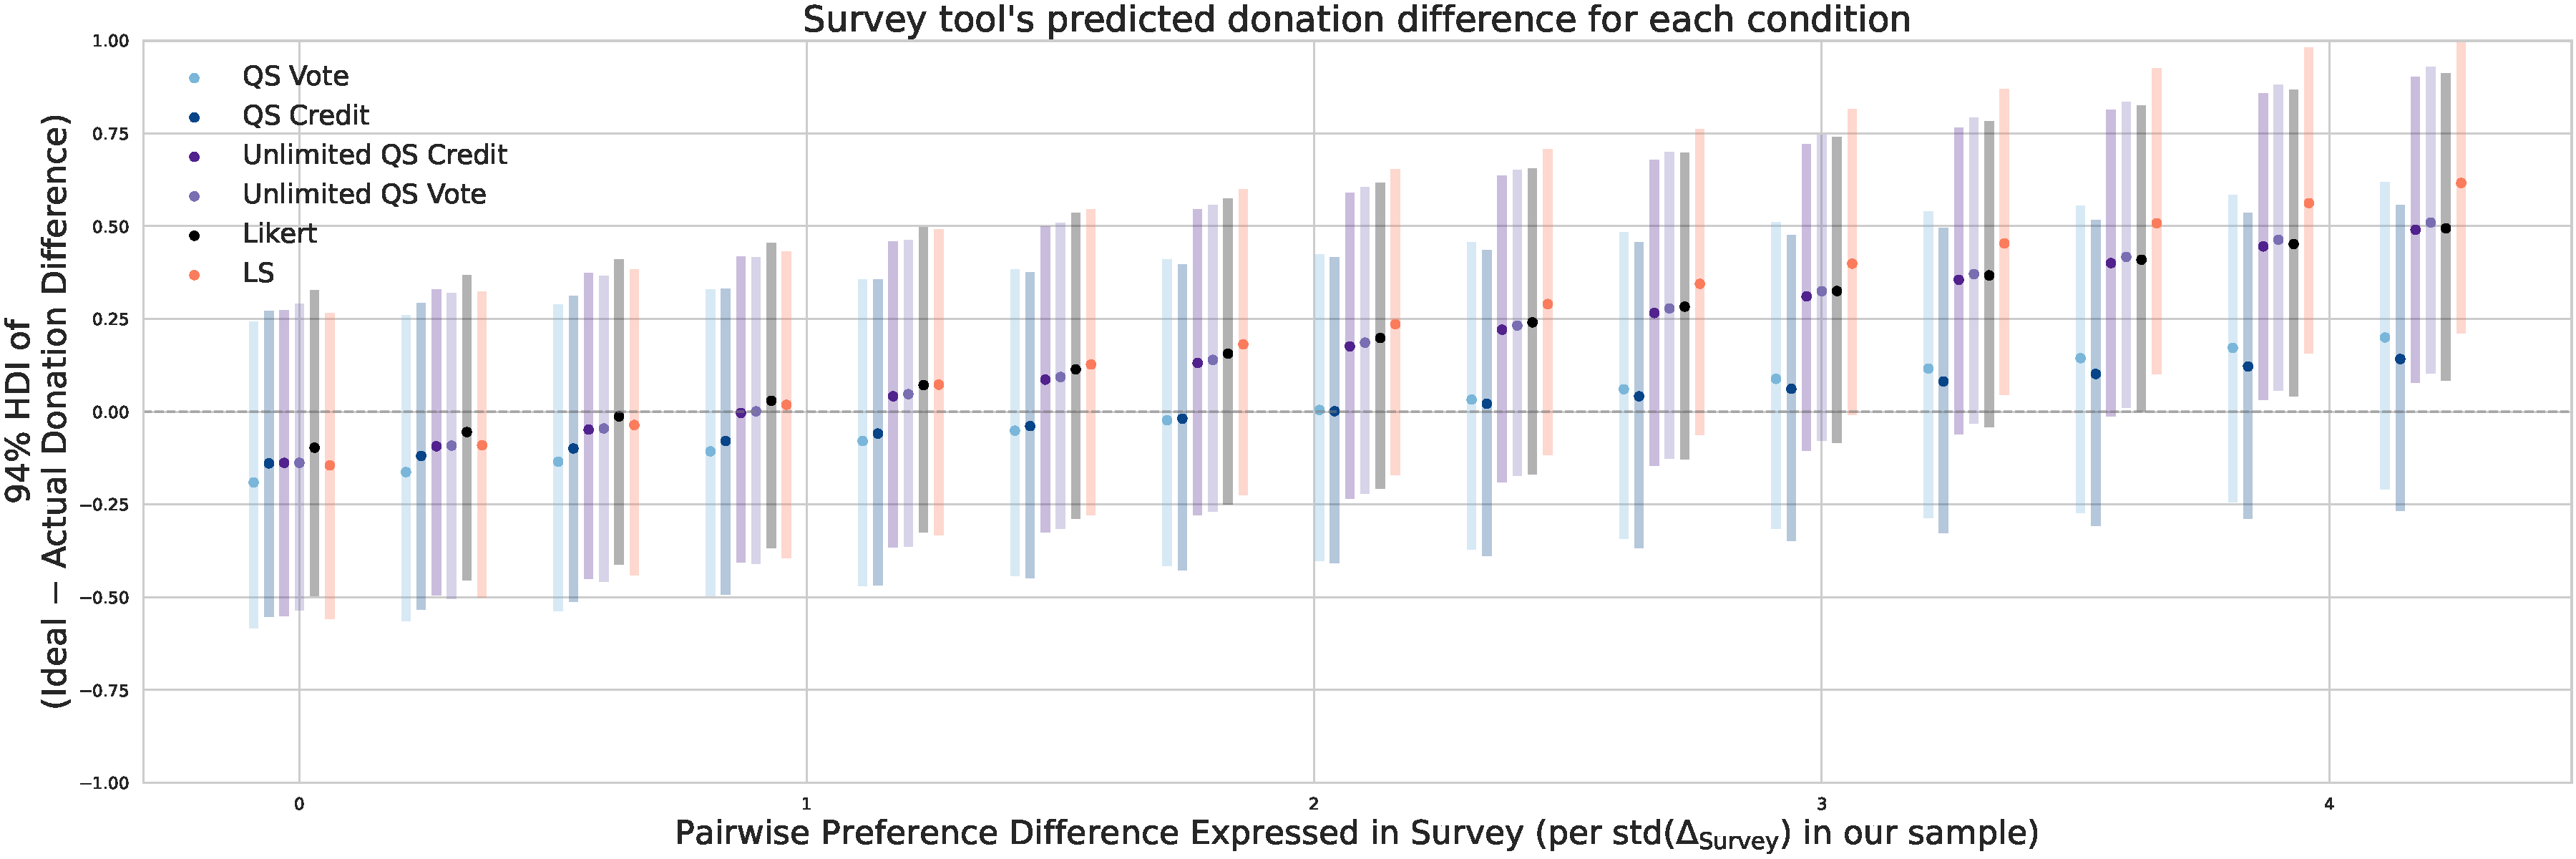
\includegraphics[width=\textwidth]{content/image/posterior_predictive_cumulative.pdf}
    \caption{Differences between survey-reported preferences and actual donation behaviors across survey tools. Dots represent mean normalized differences, with bars showing the 94\% Highest Density Interval (HDI). The horizontal line at 0 indicates perfect alignment; values above represent overstated preferences. QS Vote and QS Credit consistently show close alignment even as actual behavioral differences increase, while Likert, LS, and Unlimited QS increasingly deviate at larger differences. \textbf{Takeaway}: QS methods (Vote and Credit) better capture participants' actual preference intervals, especially as intensity differences grow.}
    \label{fig:comparison}
\end{figure*}

\subsection{Mechanisms underlying QS's effectiveness}
This subsection explores the plausible mechanisms underlying QS's effectiveness. While our results replicate and extend the observed advantage of QS over Likert scale surveys~\cite{chengCanShowWhat2021}, we focus this subsection on two mechanisms: (1) how the quadratic cost function aligns preferences with behavior, and (2) how budget constraints shape expression. We examine these mechanisms using LS and UQS results.

\subsubsection{Quadratic cost function corrects perception distortion and bias in response strengths}
As discussed in~\Cref{sec:interval_measures}, QS credits and votes remain aligned with participants' revealed behaviors across varying levels of preference strength. In contrast, our model shows increased exaggeration in LS and Likert scale survey results as the pairwise donation difference widens (see~\Cref{fig:comparison}). We identify two plausible explanations.

\paragraph{Unequal~\textit{perceived} `preference units'}
We define a 'preference unit' as the incremental amount a participant uses to express additional preference (e.g., an extra vote, extra credits spent, or an extra level on a Likert scale). Our results indicate that LS participants perceive successive preference units as representing smaller incremental differences in strength. This pattern aligns with the Law of Diminishing Marginal Utility in economics~\cite{gossen1983laws, kahnemanProspectTheoryAnalysis1979}, which states that each additional unit of consumption yields less utility than the one before. Thus, survey respondents allocate more preference units to express their intended preferences.

Even if participants do not explicitly interpret preference units in monetary terms, psychophysics offers similar concepts. According to the Weber-Fechner law~\cite{dehaeneNeuralBasisWeber2003, kruegerReconcilingFechnerStevens1989}, the just noticeable difference between stimuli is proportional to the baseline stimulus intensity. As the marginal difference between options appears to shrink, participants may feel their previous input was insufficient and overcorrect as a result. Early CSS validation by~\citet{dudekValidityPointAssignmentProcedure1957} cautioned that participants may misjudge how well their numerical input reflects their subjective attitudes. Interestingly, Fechner's law~\cite{kruegerReconcilingFechnerStevens1989} describes perception as following a logarithmic curve, which conceptually aligns with the quadratic cost structure in QS. In QS, the rising cost of additional votes may have corrected participants' diminishing perceptual increments, helping to mitigate exaggerations in expressed preferences stemming from participants' perceptual biases.

\paragraph{Extreme response bias}
Another plausible explanation involves the large decision space and the ease of expressing extreme opinions offered by LS. With the same budget size, participants face a wider array of allocation choices when votes incur a linear cost than a quadratic cost (e.g., 324 choices in LS162 vs. 25 choices in QS162 on an option). The psychology literature suggests that cognitive overload leads to satisficing~\cite{schwartzMaximizingSatisficingHappiness2002, iyengarWhenChoiceDemotivating2000}, where individuals settle for sufficient rather than optimal choices by relying on heuristics. As the allocated budget increased, participants increasingly underutilized their budgets, a pattern consistent with satisficing behavior~(\Cref{fig:credit_usage_descending}). With a satisficing mindset, rather than carefully weighing and quantifying the differences between options, participants may resort to exaggerating responses to signal distinctions between choices. While this exaggeration strategy is possible with both LS and QS, it was discouraged by the quadratic cost structure in QS. The quadratic cost function imposes increasing costs for each additional vote, which makes people think twice before expressing strong opinions. In LS, on the contrary, it does not cost much to exaggerate preferences since each vote carries equal weight. In summary, the quadratic cost structure in QS may have reduced the occurrences of exaggerated responses by alleviating cognitive load and imposing a higher cost to expressing extreme opinions.
% which lets individuals redistribute credits freely, since each vote carries equal weight. As the LS budget increases, the space of possible allocations grows rapidly. Consider LS18 and QS324, which both permit up to 18 votes~\footnote{Assuming all credits are allotted to a single option, 324 credits allows at most 18 votes which is equivalent to LS18.}; however, in QS, casting 18 votes incurs a significantly higher cost.  sharply narrowing the decision space and discouraging exaggerated responses.

\begin{figure}[ht]
  \centering

  \begin{minipage}[t]{0.48\textwidth}
    \centering
    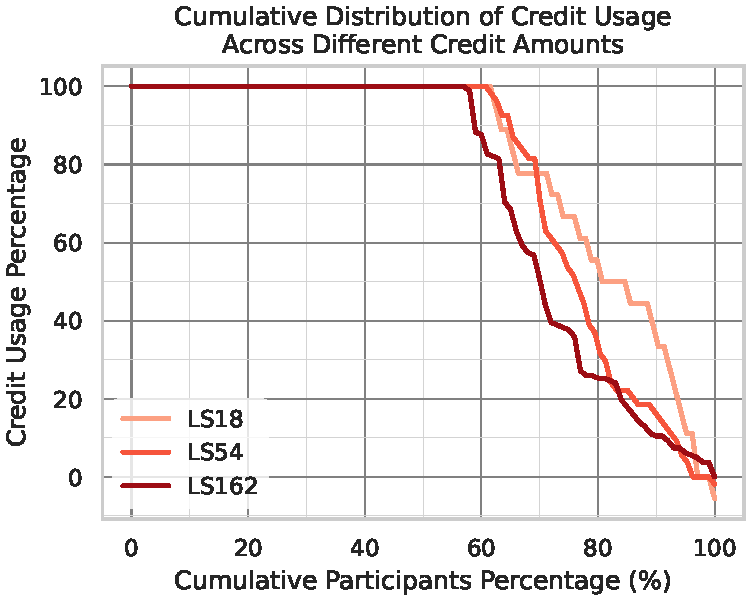
\includegraphics[width=\textwidth]{content/image/cumulative_distribution_credit_usage.pdf}
    \caption{
    Percentage of participants who fully utilized their credits across budget levels. As budgets increase, cumulative usage drops off more steeply.
    \textbf{Takeaway:} Higher budgets lead to earlier and more widespread underutilization of credits.
    }   
    \label{fig:credit_usage_descending}
  \end{minipage}
  \hfill
  \begin{minipage}[t]{0.48\textwidth}
    \centering
    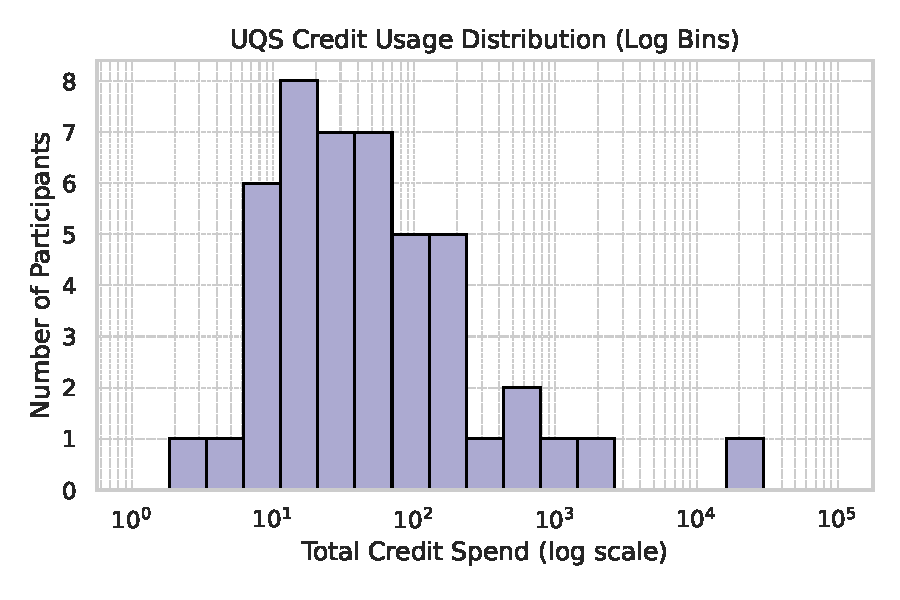
\includegraphics[width=\textwidth]{content/image/uqs_credit_usage_distribution_logbins.pdf}
    \caption{The credit usage distribution for UQS participants. The credit usage follows a long tail. Without an anchor, less than half of participants spend more than 38 credits across 9 options. \textbf{Takeaway:} Participants did not put in enough effort to use as many credits as needed to express nuanced differences between option preferences.}
    \label{fig:uqs_usage}
  \end{minipage}

\end{figure}


\subsubsection{The quadratic cost function reduces the cognitive burden influencing pairwise rankings}
This expanded decision space may have also undermined LS's ability to preserve pairwise rankings that are consistent with participants' opinions. The linear cost in LS increases the number of possible allocation outcomes compared to QS with the same budget size, raising the cognitive demand required to maintain consistent relative preferences. In contrast, QS's quadratic cost structure progressively narrows this decision space, easing the cognitive burden and facilitating more consistent preference rankings. This cognitive burden likely contributes to noisier and more inconsistent pairwise rankings. %This likely contributes to noisier and more inconsistent survey pairwise rankings. When a participant allocates $x$ votes to one option, they face a wide range of subsequent options (e.g., $x+1$ to the remaining budget) to express stronger preferences elsewhere. 

\subsubsection{The role of Budget: Anchor and a Sense of Scarcity}
UQS performs similarly to LS, likely due to two key factors. First, without a fixed budget, participants face unlimited allocation options, eliminating clear opportunity costs and tradeoffs. This can result in more extreme allocations or exaggerated expressions (e.g., one participant allocated 105 votes to a single option). Second, without a budget constraint, participants lack a stable reference for a 'preference unit,' since the meaning or weight of each additional vote shifted with each allocation. This undermines anchoring~\cite{daniel2017thinking, tverskyJudgmentUncertaintyHeuristics1974}, often necessary for initiating preference construction~\cite{lichtensteinConstructionPreference2006}, and further expands the decision space. We observe that less than half of the participants spend more than 38 credits, followed by a long tail of credit usage (\Cref{fig:uqs_usage}), possibly due to cognitive overload or because they felt further input was unnecessary. This behavior constrained the expansive decision space, suggesting that budget limits may help regulate expressive intensity.

\paragraph{In summary,} QS's quadratic cost function helps mitigate distortions caused by perceptual biases and choice overload, particularly when participants express large differences between options. The fixed budget constraint anchors participants' interpretations of preference units and limits the decision space, thereby reducing cognitive load and supporting more accurate expression.

Together, these mechanisms likely explain why QS aligns more closely with participants' behavioral outcomes than the alternatives. While each mechanism is grounded in prior literature and supported by our findings, their interaction remains unclear. Perceptual distortion, overload, and anchoring may be interdependent rather than isolated effects. Future research should investigate how participants' internally valued preferences map onto their expressed responses in QS. Cognitive interviews aimed at constructing mental models could reveal how participants interpret budget constraints, cost structures, and manage preference tradeoffs during preference construction.

\subsection{Takeaways for QS practitioners}
Our findings offer practical implications for practitioners using QS to elicit preferences in collective intelligence settings:

\paragraph{Balancing simplicity and accuracy for basic ranking tasks}
Likert scale surveys may suffice for simple rankings that do not require aggregation, given their simplicity. While QS still yields slightly better alignment with behavioral outcomes, the added complexity may not be justified in low-stakes or ordinal-only contexts.

\paragraph{QS excels in capturing preference intensity and enabling aggregation}
QS is particularly effective for capturing nuanced differences in preference strength across competing options and aggregating those preferences across individuals. Our results demonstrate that QS significantly outperforms traditional methods in capturing preference intensities and enabling aggregation.

\paragraph{Do not compromise the QS mechanism}
Both the quadratic cost function and the budget constraint are essential for QS to function effectively. Removing either component (as in LS or UQS) substantially reduces performance. Since these features introduce cognitive load, it is essential to design usable interfaces that support participants' preference construction process.

\paragraph{Credit budget matters less, but a medium range is recommended}
Although we observed no statistically significant differences among QS36, QS108, and QS324, Bayesian analysis consistently favored QS108 for stable, balanced outcomes. Thus, practitioners are advised to scale the credit budget to the power of 1.5 relative to the number of options ($O(k^{1.5})$ as defined by prior research~\cite{chengCanShowWhat2021}.

\section{Limitations and Future work}
\label{sec:limitations}

\paragraph{Limitations of donation-based preference elicitation}
Behavioral donation tasks are widely used in prior research~\cite{xiao2019should, gendall2010effect, benz2008people, chengCanShowWhat2021} to approximate ``true preferences'' through real-stakes decisions for survey validation. While the donation task in this study was adapted from prior designs to ensure incentive compatibility and behavioral realism, not all preferences are naturally expressed through monetary contributions. Participants' mental models, shaped by donation amounts, prior giving, or personal motivations, may differ from those guiding their responses to survey instruments. Moreover, although charitable donations offer incentive-aligned behavior, the domain involves distinct social and motivational factors that may not generalize to other allocation contexts. Governmental resource allocation, for instance, includes political accountability, public transparency, and long-term planning considerations. Future field studies applying QS in public decision-making settings could further assess its generalizability.

\paragraph{Future work: comparing QS with other forced-choice methods}
The limited performance of LS highlights the need for future comparative studies between QS and other forced-choice preference elicitation tools, such as KS and conjoint analysis. These methods rely on different constraints and mechanisms to reveal preference intensity. Comparing them across decision contexts and preference distributions would help practitioners identify the most appropriate tools. Future evaluations should consider elicitation accuracy, cognitive load, and user experience.
